\documentclass[11pt, oneside]{article}   	% use "amsart" instead of "article" for AMSLaTeX format
\usepackage{geometry}                		% See geometry.pdf to learn the layout options. There are lots.
\usepackage{textcomp}
\usepackage{hyperref}  % TODO: see page 94 of latex book
\geometry{letterpaper}                   		% ... or a4paper or a5paper or ... 
%\usepackage[parfill]{parskip}    		% Activate to begin paragraphs with an empty line rather than an indent
\usepackage{graphicx}				% Use pdf, png, jpg, or eps§ with pdflatex; use eps in DVI mode
								% TeX will automatically convert eps --> pdf in pdflatex		
\usepackage{amssymb}
\usepackage{amsmath}
\usepackage{relsize}

\title{CSCI 181 / E-181 Spring 2014 Practical 3 \\ 
{\large Kaggle Team "Capt. Jinglehiemer"}
}
\author{
  David Wihl\\
  \texttt{davidwihl@gmail.com}
  \and
  Zack Hendlin\\
  \texttt{zgh@mit.edu} 
}
%\date{}							% Activate to display a given date or no date

\begin{document}
\maketitle
\section*{Warm-Up}

We consider two approaches for classifying fruits (with length and width measurements provided) into one of three categories.

It is important to note that the data here is not perfectly linearly seperable, as can be seen in the plot below:

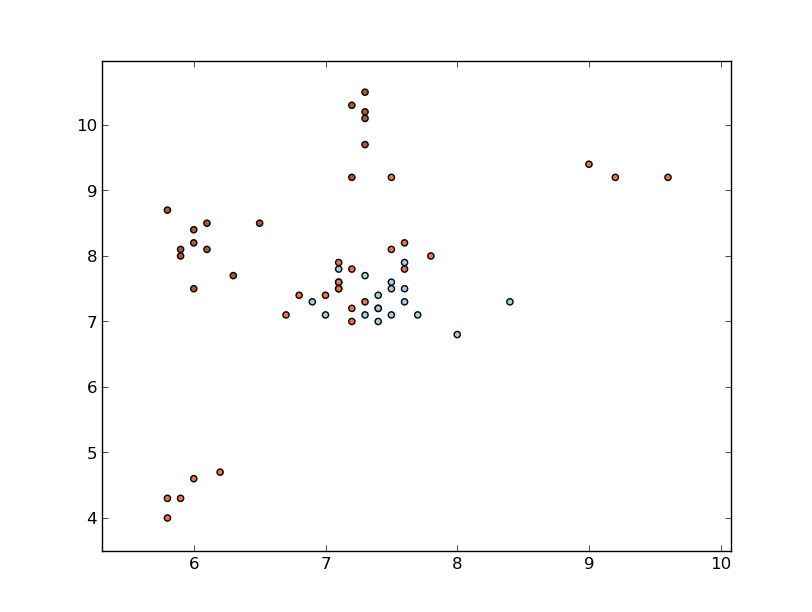
\includegraphics[scale=.6]{figure_3}

So the challenge becomes how we can best define mutually exclusive regions of the graph.

\subsection*{Logistic Classification}

Multiclass logistic classification seeks to define the weights that minimize:
\\
 $E(w_1, w_2, ..., w_K) =  -\sum\limits_{n=1}^N \sum\limits_{k=1}^K = t_{nk} ln_{nk}$ , 
as given in equation 4.108 in Bishop.
\
\\
Here our $w$ vector will have be $k x 3$ as we have a variable for height, weight, and then an offset term $w_0$.
\
\\
Since $k=3$, we fit 9 weights so as to minimize the error function. We use the Broyden Fletcher Goldfarb Shanno algorithm (BFGS) as implemented in the Scipy package. We select this because it provides a better approximation to the Hessian at each step.
\
\\
The error function achieves its minimum at 34.769598, and takes 44 iterations to converge.
\\
Once we have the weights:

\[
w=
  \begin{bmatrix}
    -7.35269067 & 2.48983592 & -1.17947522\\
    -3.65199071 & 1.66456348 & -0.81582258\\
    14.00478476 & -4.15564072 & 1.99410538\\	
	
  \end{bmatrix}
\]
\\
\
 we then use in the softmax function:
\
$y_k(\phi) = exp(a_k)/\sum\limits_{j=1}^K exp(a_j)$
\\
where $a$ is simply the dot product of $x$ and $w$,to evaluate which class has the highest likelihood for a particular data point. The point is then assigned to the class which has the highest class-conditional density.
\\
We get the resulting classification.

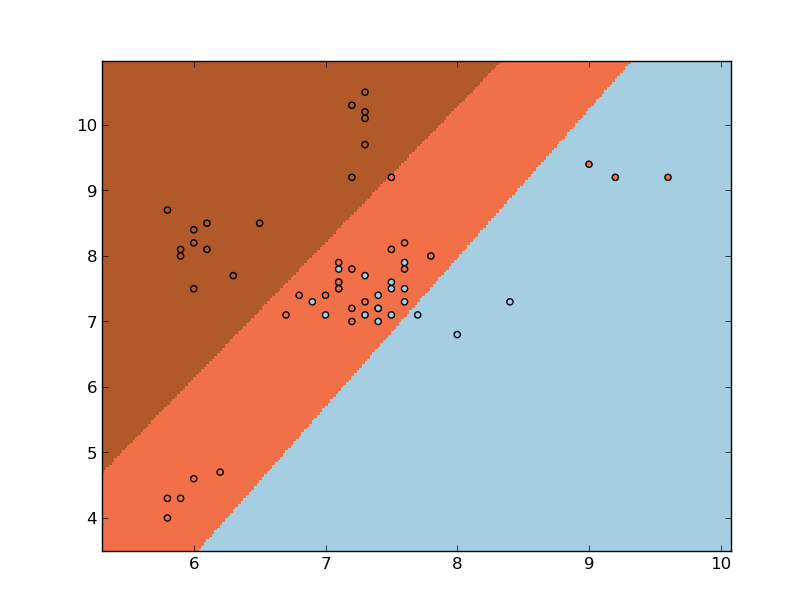
\includegraphics[scale=.6]{logistic_classifer}

\subsection*{Generative Model Classification}

Generative models attempt to determine, for each class $k$, a likelihood that a data point is generated by that particular class.
\\
\ We first calculate the prior likelihoods for each class $P(c_k)$
\\
\ And then recognizing we want $p(C_k |x_n)$ by applying Bayes rule, we need: $p(x_n |C_k)$.
\\
The multivariate normal is given by:
\
\\
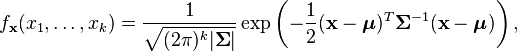
\includegraphics[scale=.5]{formula}
\
\\
where k=2 in our case because we have (1) height and (2) width.
\
\\
This gives us a probability density function for each class. We then apply Bayes rule:

$p(C_k |x_n) = p(x_n |C_k)  p(C_k) / \sum\limits_{j=1}^K p(x_n | c_j) * p(c_j)$

and note that we can ignore the denominator since it is the same for all classes.

\\
We then have an assignment for each point to the highest likelihood class as shown in plot below.
\\
\
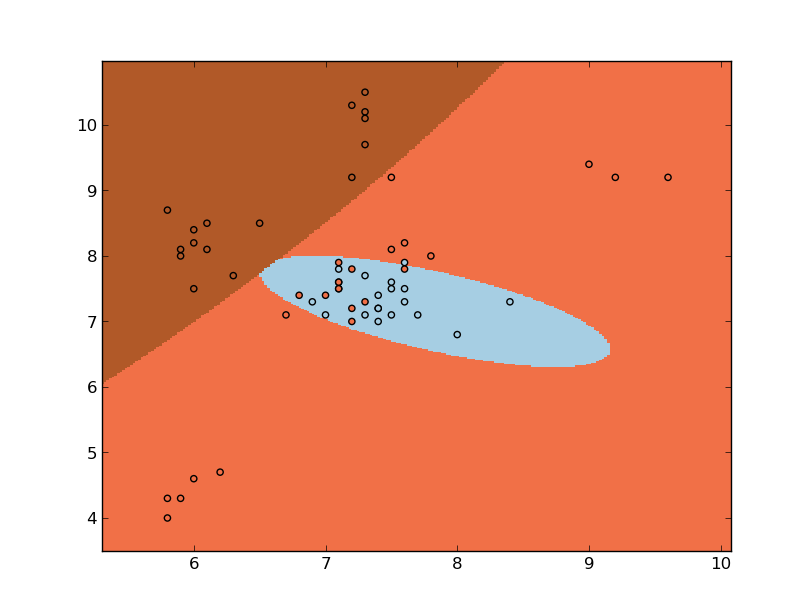
\includegraphics[scale=.6]{generative_classifier}


\subsection*{Warmup Summary}

As we can see from the graphs in the previos sections, allowing a non-linear decision boundry (as we did when we used the generative classifier) allowed more flexibility to capture clusters of points and indeed was more accurate at capturing the variation observed in the data.

\section*{Classifying Malicious Software}

\subsection*{Preliminary Data Analysis}

As soon as we started the analysis the large 4GB XML file size was causing issues in parsing and processing. To ameliorate this, we first split the training and the testing. This allowed us to use only the relevant train/test data at each step, reduced file size and computation time, and also enabled parallelization of test runs over a cluster of machines. We shared this code on Piazza for the benefit of other students.

\subsection*{Using Cross-validation}
Five-fold cross validation was used on the training data, with runs with train / CV data pairings of 70/30, 80/20 and 90/10 for each classifier.

This was valuable in helping to reduce the risk of overfitting, and was useful in obtaining more robust results.

\section*{Approaches considered}

We actually found that combining two different sets of classifers worked under different situations. For instance, we found that the summary features had the most overall explanatory power (XX percent), but that more specific information on each process was useful in specifically identifying certain cases.
\
\\
Interestingly, we found that the hyper-detailed information on each process feature was actually less useful on average than more aggregated features. This points to the importance of feature engineering and trying to capture key elements of the underlying data rather than simply adding features without as much thought to why they might make sense and if they are the best representation of key attributes.
\
\\
While we initially had them as seperate models, we instead developed a 'meta classifier' which we trained to simply discriminate which of the two models was likely to perform well on that type of potential malware. We used this model to then select between the two model prediction



\subsection*{Feature Engineering}

NOTE
Aggregate Features per training file:
 selected all process features  (e.g. 'startreason', 'terminationreason', 'username', 'executionstatus', 'applicationtype') and summary thread features (num of each type of system call).

used CV to generate Logistic Regression weights. Took mean and std of resulting matrix, then eliminated any features where abs(mean) $<$ 0.001 and std $< $0.01.



\subsection*{Selection of fitting technique}
NOTE
We explored Logistic Regression and SVM with a range of different C values, but this range in C values didn't make a significant difference.


\subsection*{Exploratory Data Analysis}
NOTE

\section*{Conclusion}
\\
We conclude from this practical that considering what classifiers work well over what ranges is extremely important. That is, when we combined models to allow them to effectively apply over different 'ranges' of the data, we were able to capture more nuanced effects than if we had simply attempted a single set of classifers that was applied to all data across the range. 
\\
\
This idea -- which is also true in decision trees and random forests -- effectively allows the function mapping the data to be more specific to the variability observed in the data and points to an important idea for us to consider in future machine learning projects.

\end{document}  
